\subsubsection{Projection of Run-2 CMS searches for a new scalar resonance decaying to a pair of Z bosons}
\begin{center}
 {\it{ by Meng Xiao}}
\end{center}

\subsubsubsection{Introduction}
CMS and ATLAS collaborations have performed searches for a heavy scalar partner of the SM Higgs boson decaying into a pair of Z bosons~\cite{Aaboud:2018bun,Sirunyan:2018qlb}. The CMS search for a heavy scalar partner of the SM Higgs boson using $35.9 \mathrm{fb}^{-1}$ of pp collision data~\cite{Sirunyan:2018qlb} will be referred to as HIG-17-012 throughout this section. In HIG-17-012, the search for a scalar resonance $\PX$ decaying to $\PZ \PZ$ is performed over the mass range $130\UGeV < m_{\PX} < 3$\UTeV, where three final states based on leptonic or hadronic decays of Z boson, $\PX\to \PZ\PZ\to 4\ell$, $2\ell2\Pq$, and $2\ell2\nu$ are combined. Because of the different resolutions, efficiencies, and branching fractions, each final state contributes differently depending on the signal mass hypothesis. The most sensitive final state for the mass range of 130--500\UGeV is $4\ell$ due to its best mass resolution, whereas, for the intermediate region of 500--700\UGeV, $2\ell2\nu$ is most sensitive. For masses above 700\UGeV the $2\ell2\Pq$ provides the best sensitivity. In this paper, we are particularly interested in the sensitivity in the high mass region, thus only $2\ell2\Pq$ is used. 

In the $2\ell2\Pq$ final state, events are selected by combining leptonically
and hadronically decaying \PZ\ candidates. The lepton pairs (electron or muon) of opposite sign and same flavor 
with invariant mass between 60 and 120 GeV are constructed.
Hadronically decaying $\PZ$ boson candidates are reconstructed using two distinct
techniques, which are referred to as ``resolved'' and ``merged''.
In the resolved case, the two quarks from the $\PZ$ boson decay form two distinguishable narrow jets, while in the merged case a single wide jet with a large $p_T$ is taken as a hadronically decaying Z candidate.

The two dominant production mechanisms of a scalar boson are gluon fusion (ggF) and EW production, the latter dominated by vector boson fusion (VBF) with a small contribution of
production in association with an EW boson ZH or WH (VH). We define the parameter $f_{VBF}$ as the fraction of the EW production cross section with respect to the total cross section. The results are given in two scenarios: $f_{VBF}$ floated, and $f_{VBF}=1$. In the expected result, the two scenarios correspond to ggF and VBF production modes, respectively. To increase the sensitivity to the different production modes, events are categorized into VBF and inclusive types. Furthermore, since a large fraction of signal events is enriched with \PQb\ quark jets due to the presence of $\PZ\to\PQb\PAQb$ decays, a dedicated category is defined.

The invariant mass of $\PZ \PZ$ and a dedicated discriminant separating signal and background distributions are compared between observation and expected background to set limits on the production cross section. 

Further details of the HIG-17-012 analysis, including simulation samples, event categorisatoin, background estimation methods, systematic uncertainties, and different interpretations are described in Ref~\cite{Sirunyan:2018qlb}. Only details of direct relevance to the projection of the HIG-17-012 are documented in the following.

\subsubsubsection{Extrapolation procedure}

A projection of this analysis is carried out by scaling all the signal
and background processes to an integrated luminosity of 3000$\mathrm{fb}^{-1}$, expected to be collected at the high-luminosity LHC. This projection assumes that the CMS experiment will have a similar level of detector and triggering performance during the HL-LHC operation as it provided during the LHC Run~2 period. It does not take into account the small cross section change due to the small change in the center of mass energy from 13 TeV to 14 TeV. The results of projection are presented for different assumptions based on the size of systematic uncertainties that is estimated for HL-LHC. %More details are given in the previous Section~\ref{sec:XZZ}.

\subsubsubsection{Results}
\begin{figure}[htbp]
        \centering
                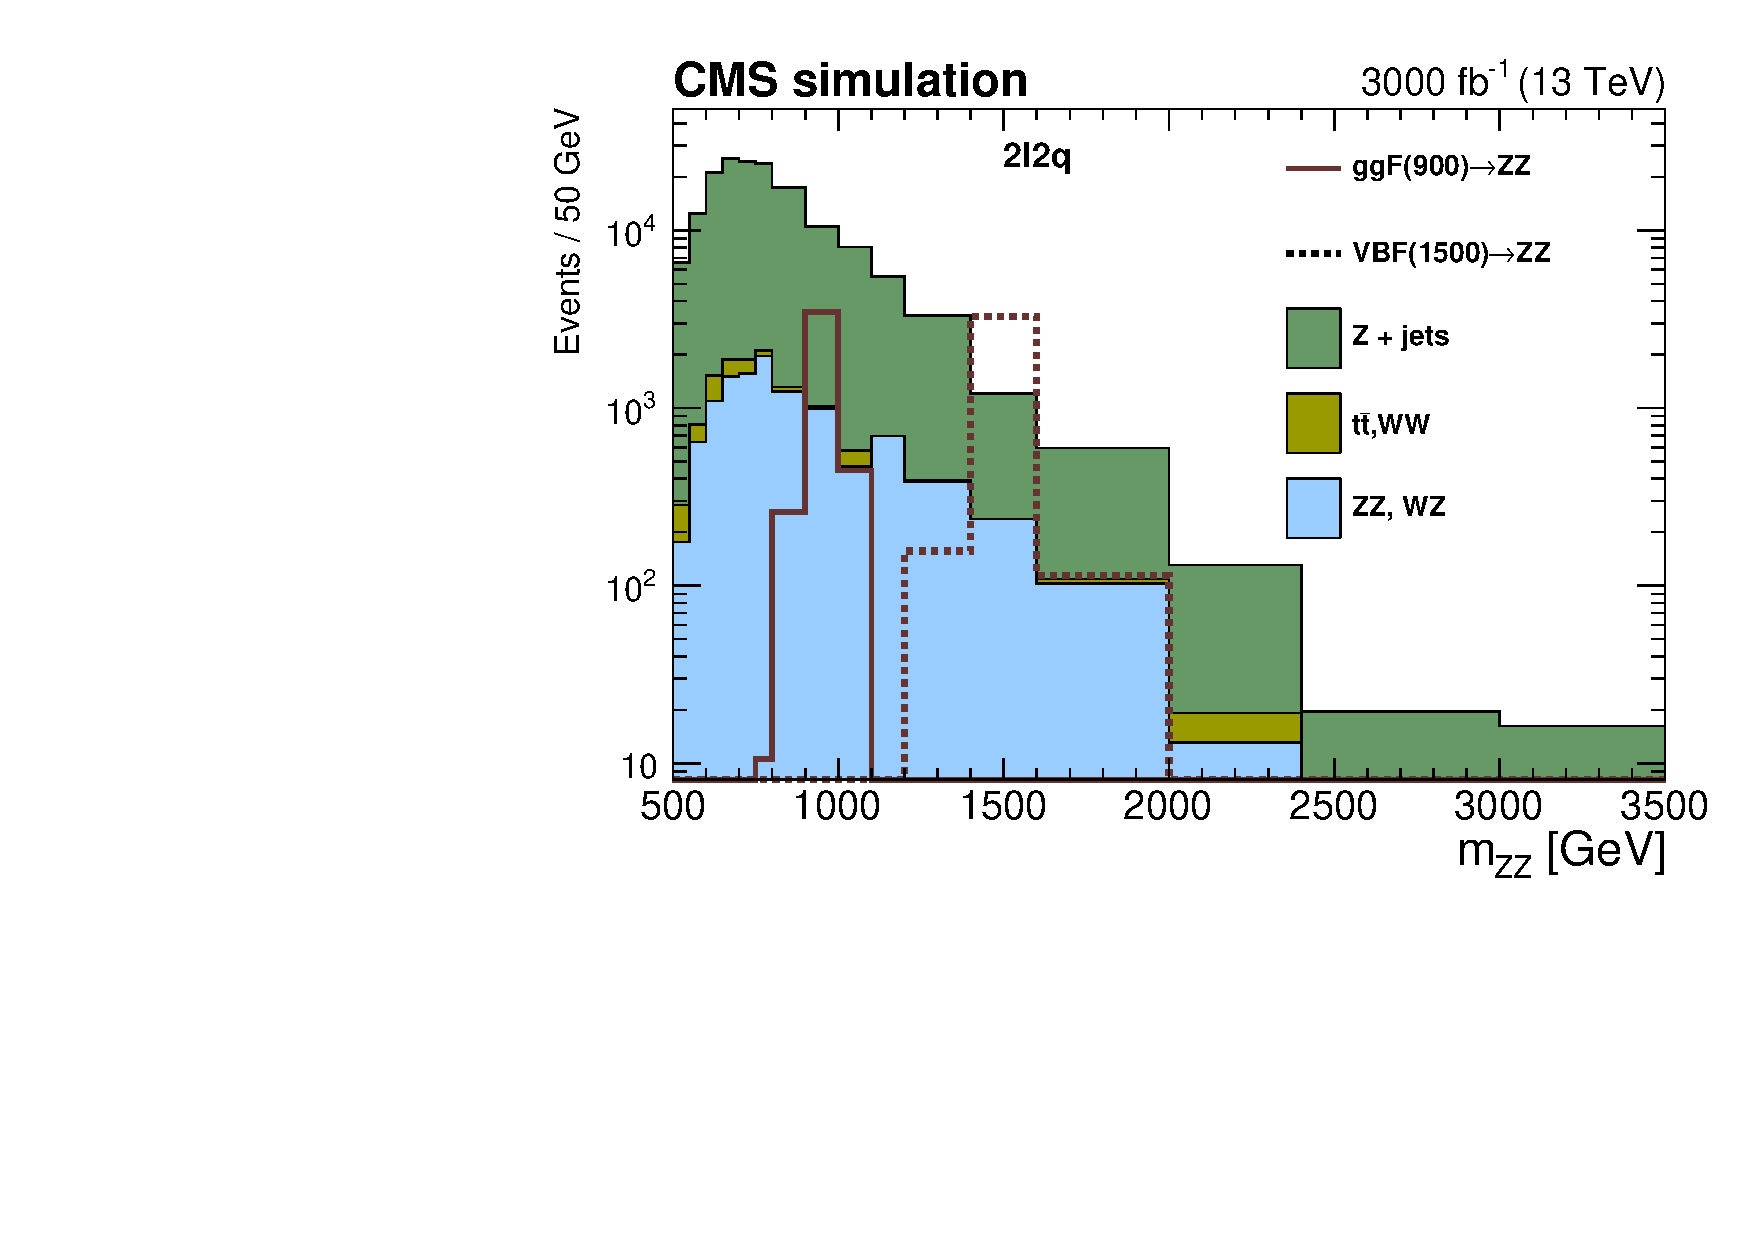
\includegraphics[width=0.48\textwidth]{\main/section9/plots/cms_xzz/hmass_final_mergedSR.pdf}
                \caption{The $m_{\PZ\PZ}$ distribution of the merged category events expected at 3000$\mathrm{fb}^{-1}$. Examples of a 900 \UGeV ggF signal and a 1500 \UGeV VBF signal are given. the cross section corresponds to 10 times the excluded limit. 
        \label{fig:mzz}
        }
            \end{figure}
The $m_{\PZ\PZ}$ distribution of the merged category events expected at 3000 $\mathrm{fb}^{-1}$ is shown in Figure~\ref{fig:mzz}. Figure~\ref{fig:combinedresult} shows upper limits at the 95\% confidence level (CL) on the $\Pp\Pp\to\PX\to\PZ\PZ$ cross section
$\sigma_{\PX} \mathcal{B}_{{\PX}\to\PZ\PZ}$ as a function of $m_\PX$ for a narrow resonance whose $\Gamma_\PX$ is much smaller than experimental resolution.

In the mass range between 550--3000 GeV, the excluded cross section of the scalar decaying to a pair of Z bosons is 0.7--5~\unit{fb} for the VBF production mode and 0.8--9~\unit{fb} for the ggF production mode. This represents a factor of 10 improvement with respect to the resuts obtained using Run 2 data. The differences between the two scenarios are minor and mostly present in the low mass region. It is because the search will still be limited by statistical uncertainties. Among all the systematic uncertainties, the theoretical uncertainty from higher order QCD corrections on the $gg\to ZZ$ background and the signal is the most dominant for the ggF search. The next important ones are the shape and yield uncertainties of the Z$+$jets background. They are determined from a data control region and are scaled with $1/\sqrt{L}$ in YR18 scenario. It is expected that at HL-LHC, the Z$+$jets background will have huge statistics, and the understanding of it will be at percent level. The effect of systematics in this search has mild effect, if no $1/\sqrt{L}$ scaling is applied, the difference in the limit is 10\% at low mass and almost none in the high mass region. In the HIG-17-012 analysis, Z$+$jets fake rates are derived from LO MC samples, and differences with repect to NLO samples are assigned as systematic uncertainty. This major source is treated as a theoretical uncertainty and is scaled by 0.5 in the YR18 scenario. 
The results for wide resonances are not given in this note for simplicity. The Run-2 result has shown that the excluded cross section for a 30\% width resonance will be 40\% higher at 1 TeV, compared to a narrow resonance assumption. 

\begin{figure}[htbp]
        \centering
        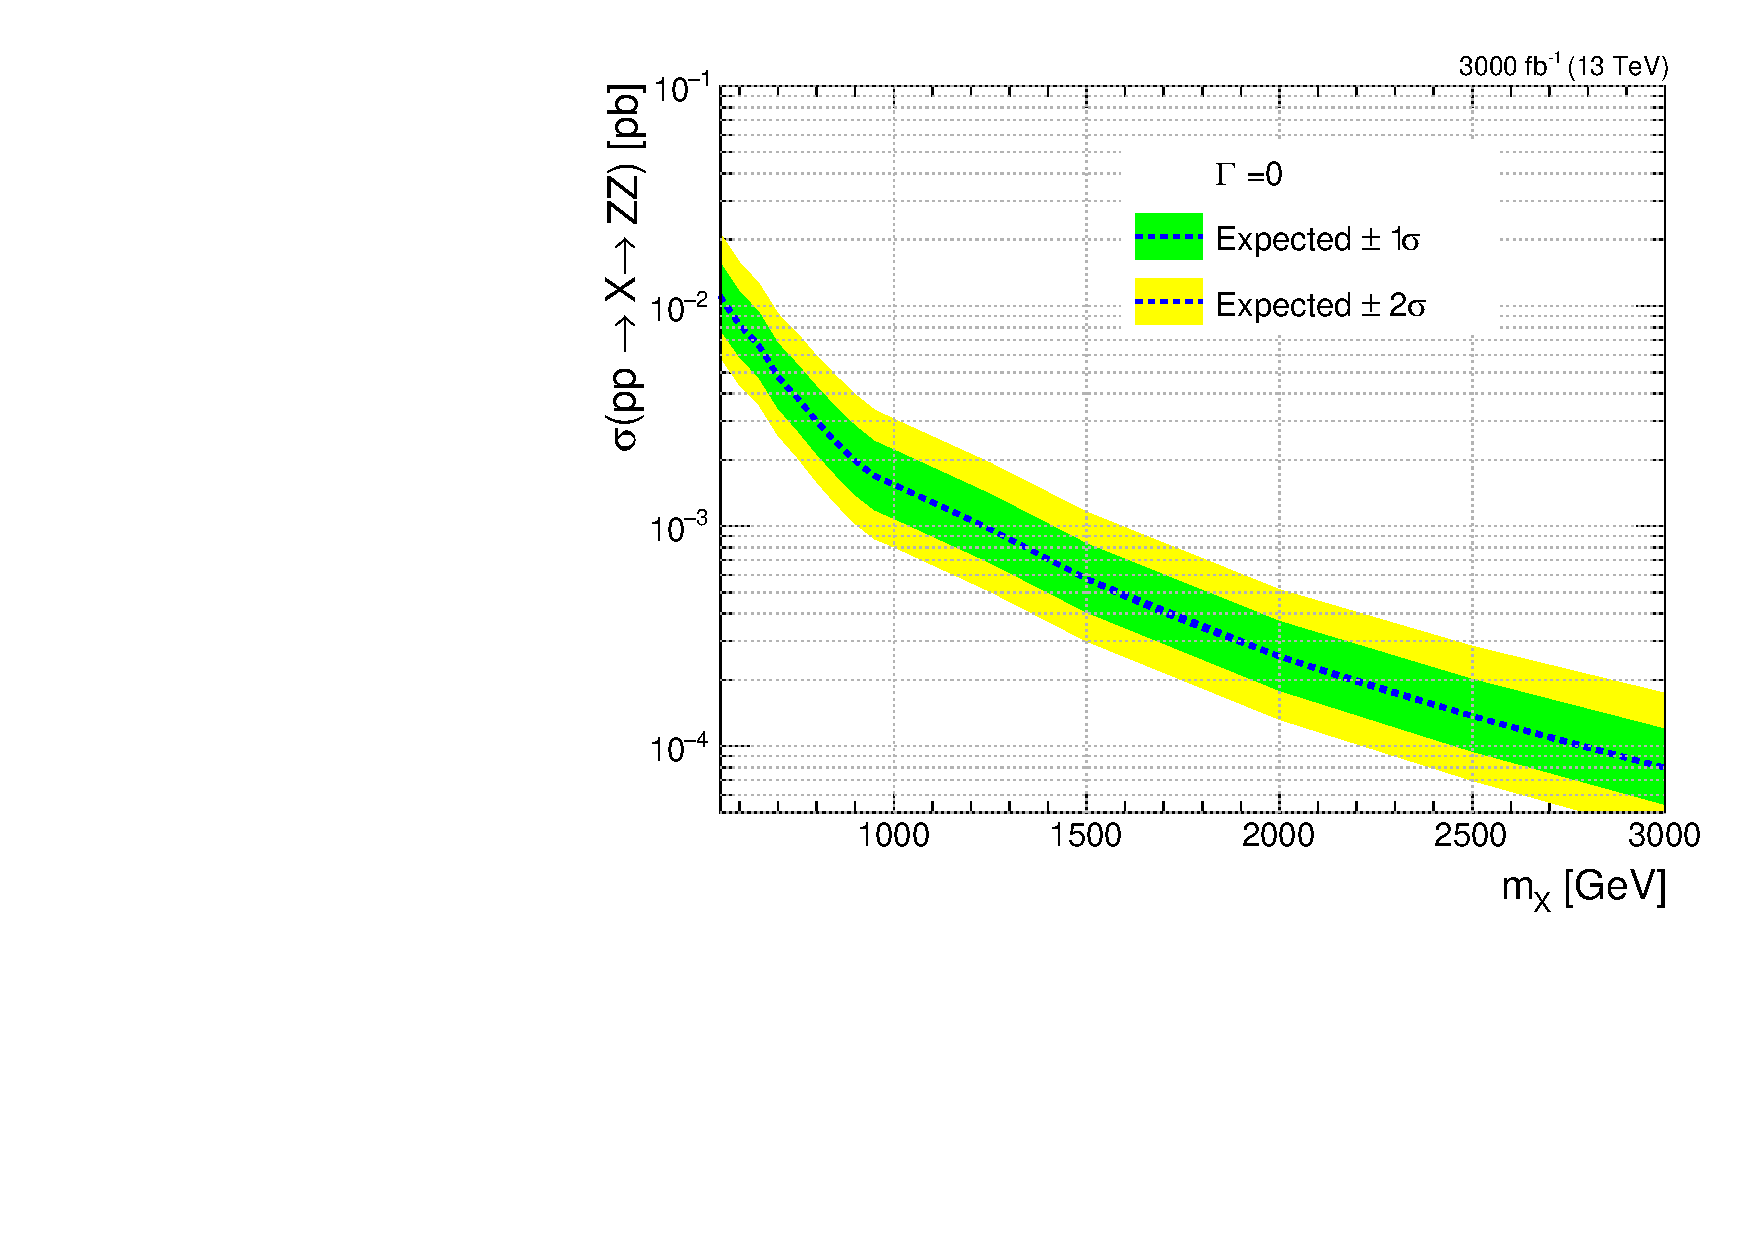
\includegraphics[width=0.48\textwidth]{\main/section9/plots/cms_xzz/2l2q_pro_2D.pdf}
        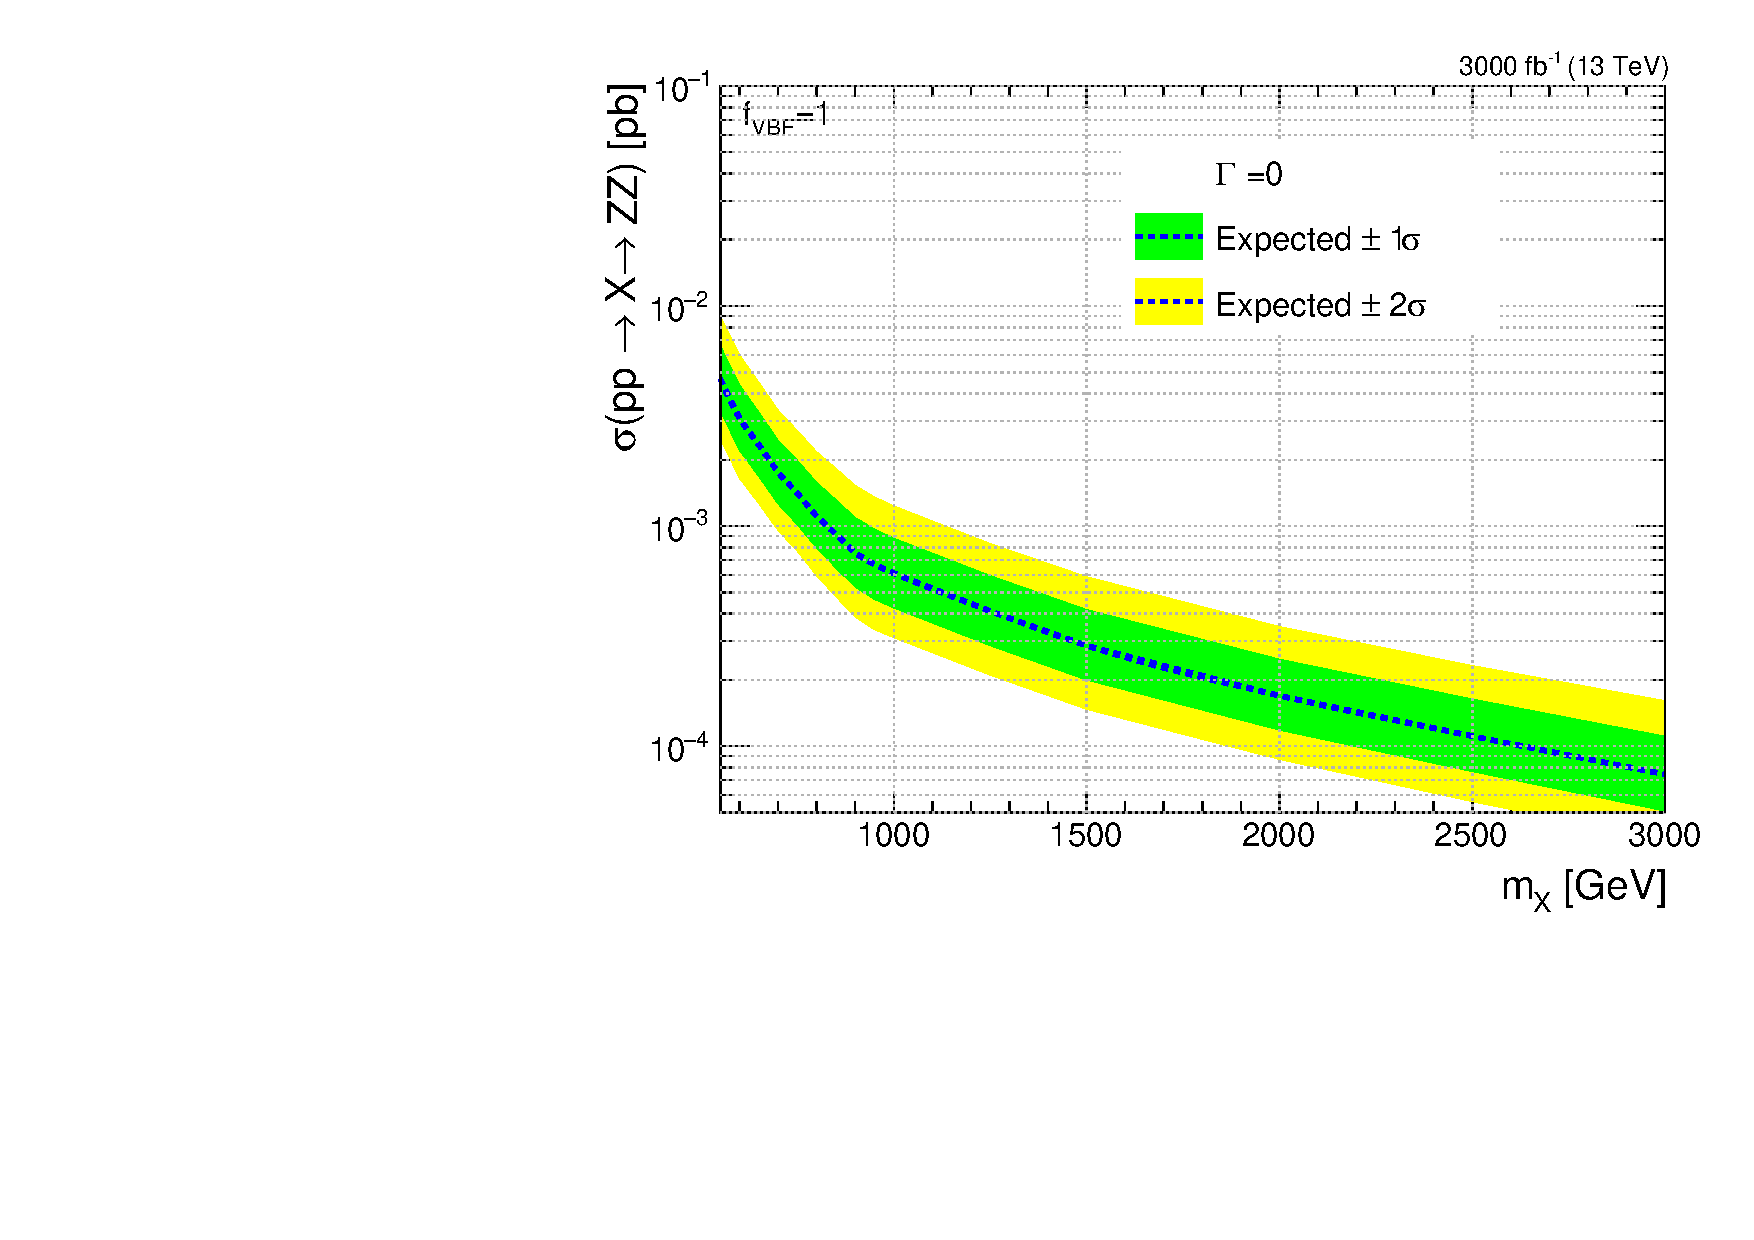
\includegraphics[width=0.48\textwidth]{\main/section9/plots/cms_xzz/2l2q_vbf_2D.pdf}\\
        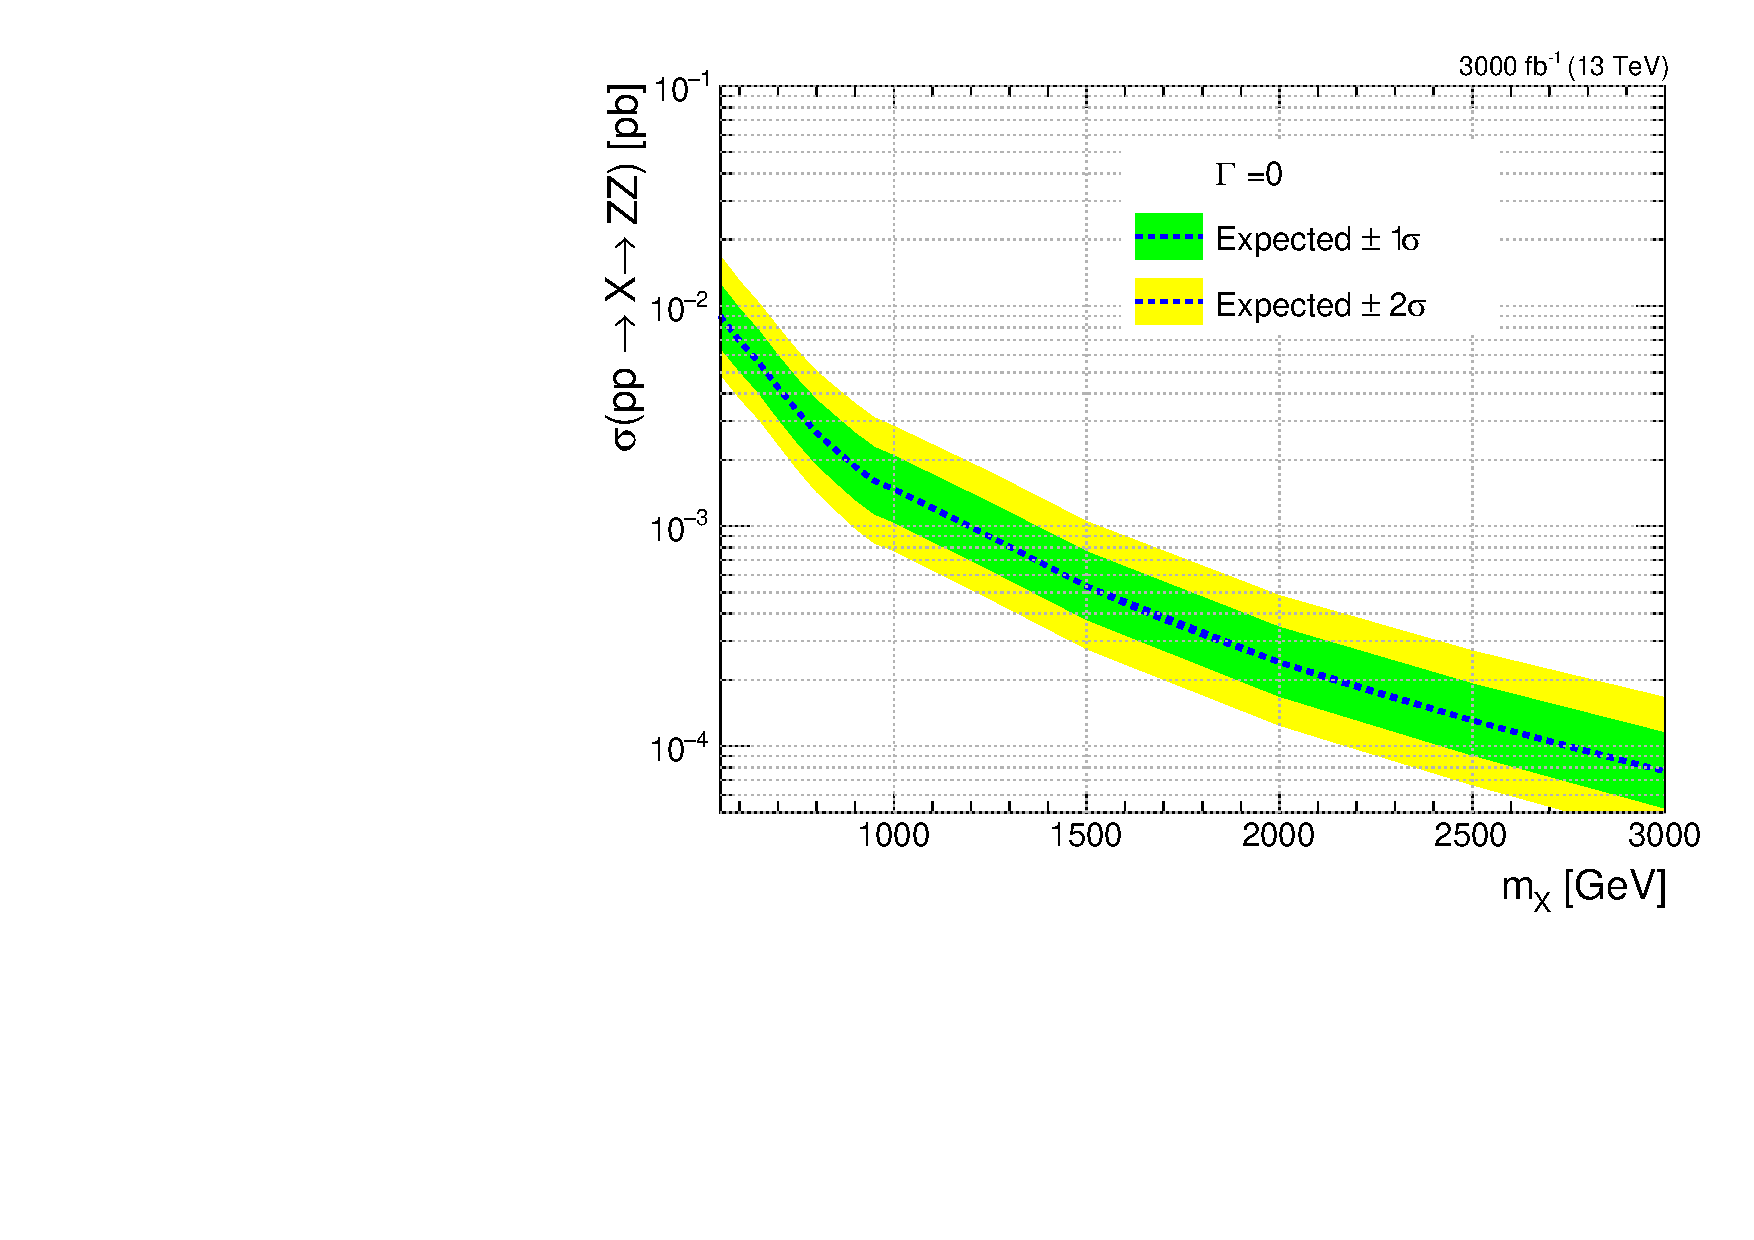
\includegraphics[width=0.48\textwidth]{\main/section9/plots/cms_xzz/2l2q_pro_scen2.pdf}
        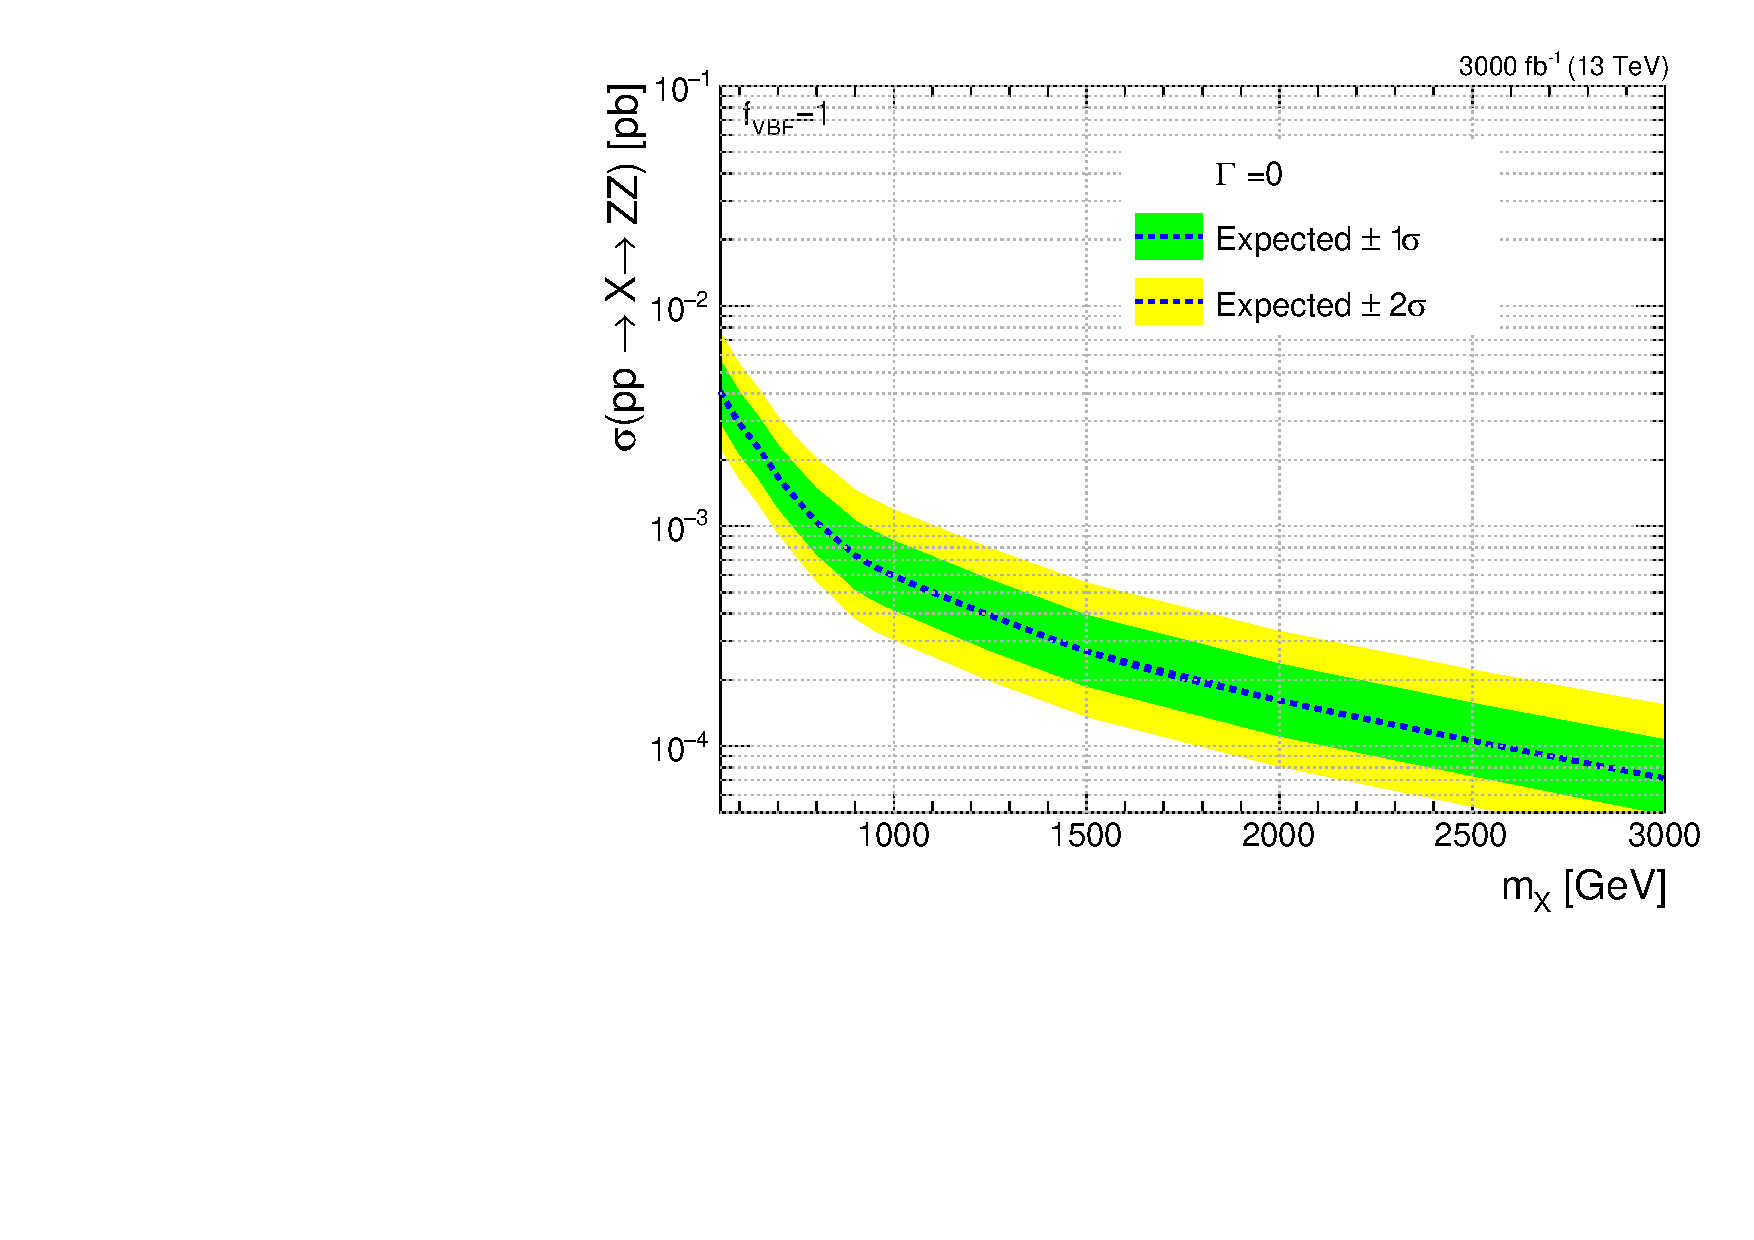
\includegraphics[width=0.48\textwidth]{\main/section9/plots/cms_xzz/2l2q_vbf_scen2.pdf}
        \caption{
                Expected upper limits at the 95\% CL on the $\Pp\Pp\to\PX\to\PZ\PZ$ cross section as a function of $m_\PX$, with $f_{\mathrm{VBF}}$ as a free parameter (left) and fixed to 1 (right). Scenario 1 (top) and scenario 2 (bottom) are shown. The scalar particle X is assumed to have a more narrow decay width than the detector resolution. The results are shown for the $2\ell2\Pq$ channel. 
                        \label{fig:combinedresult}
                }
\end{figure}